\documentclass[100,a4paperpaper,]{article}

  \title{\textbf{\textcolor{white}{Relatório de Conjuntura}}}
  \author{\textbf{\textcolor{white}{Crédito}}}
  \date{\textbf{\textcolor{white}{Outubro/2021}}}
  


\newcommand{\logo}{c:/Users/700105212/R Projects/econdashboard/inst/app/www/img/logo-banestes-transparente.png}
\newcommand{\cover}{c:/Users/700105212/R Projects/econdashboard/inst/app/www/img/cover-banestes-menor.png}
\newcommand{\logotitle}{c:/Users/700105212/R Projects/econdashboard/inst/app/www/img/logo-banestes-branca.png}
\newcommand{\iblue}{004b8d}
\newcommand{\igray}{d4dbde}
\usepackage{booktabs}
\usepackage{longtable}
\usepackage{array}
\usepackage{multirow}
\usepackage{wrapfig}
\usepackage{float}
\usepackage{colortbl}
\usepackage{pdflscape}
\usepackage{tabu}
\usepackage{threeparttable}
\usepackage{threeparttablex}
\usepackage[normalem]{ulem}
\usepackage{makecell}
\usepackage{xcolor}

% Author: Karol KozioL
% License: GPL-3
% Modified by: Sarah Wagner

% % % packages -----------------------------------------------------------------------------------
\usepackage{amsmath}
\usepackage{array}
\usepackage{booktabs}
\usepackage{calc}
\usepackage{eso-pic}
\usepackage[left = 30pt, right = 30pt, top = 25pt, bottom = 25pt, headsep = 40pt, includeheadfoot]{geometry}
\usepackage{fancyhdr}
\usepackage{fontspec}
\usepackage{graphicx}
\usepackage[utf8]{inputenc}
\usepackage{lastpage}
\usepackage{multirow}
\usepackage{tabularx} 
\usepackage{tikz}
\usepackage{titlesec}
\usepackage{titling}
\usepackage{xcolor, colortbl}
\usepackage{etoolbox}
\usepackage{ragged2e}
\usepackage{xcolor}
\usepackage[fontsize=14]{scrextend}
\usepackage[portuguese]{babel}
\usepackage{indentfirst}

% % % settings -----------------------------------------------------------------------------------

% % custom colors
\definecolor{iblue}{HTML}{\iblue}
\definecolor{igray}{HTML}{\igray}

% definition of pagename
\newcommand\pagename{Page}

% % fonts 
\defaultfontfeatures{Mapping = tex-text}
\setmainfont{Arial}
\newfontfamily\headingfont{Arial}



% % sections
\titleformat{\section}{\color{iblue}\headingfont\Large\bfseries}{\thesection}{1em}{}[\titlerule]
\titleformat{\subsection}{\color{iblue}\headingfont\large\bfseries}{\thesubsection}{1em}{}
\titleformat{\subsubsection}{\color{iblue}\headingfont\large\bfseries}{\thesubsubsection}{1em}{}

% % misc
\setlength{\parindent}{0em} 
\setlength{\parskip}{1em}
\linespread{1.15}
\renewcommand{\baselinestretch}{1.25}
\raggedright
\newcolumntype{C}{>{\centering\arraybackslash}X}
\justifying


% % % custom titlepage ----------------------------------------------------------------------------
\newcommand\BackgroundPic{%
	\put(0,0){%
		\parbox[b][\paperheight]{\paperwidth}{%
			\vfill
			\centering
			
\includegraphics[width=\paperwidth,height=\paperheight]{\cover}%
			\vfill
}}}

\makeatletter

% pagestyle titlepage
\fancypagestyle{customtitle}{
	\lhead{}
	\chead{}
	\rhead{\includegraphics{\logotitle}}
	\makeatother
	\lfoot{}
	\cfoot{}
	\rfoot{}
}


% titlepage
\renewcommand{\maketitle}{
	\thispagestyle{customtitle}
	\AddToShipoutPicture*{\BackgroundPic}
	\ClearShipoutPicture
	
	\phantom{a}\hfill
	\vspace{12cm}
	
	\begin{tabular}[l]{@{}p{\textwidth}@{}}
		\color{iblue}\headingfont\LARGE\@title\\[1em]
		\color{iblue}\headingfont\Large\@author\\[1em]
		\color{iblue}\headingfont\large\@date\\[1em]
	\end{tabular}
	
	
	\clearpage
}

\makeatother

% % % header and footer ---------------------------------------------------------------------------
\pagestyle{fancy}
\lhead{}
\chead{}
\rhead{ 
\includegraphics{\logo}}
\makeatother
\newlength{\myheight}
\lfoot{}
\cfoot{}
\rfoot{\pagename~\thepage \hspace{1pt} / \pageref{LastPage}}
\renewcommand\headrulewidth{0pt}
\renewcommand\footrulewidth{0pt}




\begin{document}


\renewcommand{\contentsname}{Sumário}


\maketitle
\tableofcontents
\clearpage

\section{Operações de crédito do Sistema Financeiro Nacional (SFN)} 
 \vspace{0.5cm}

De acordo com o Banco Central, o saldo total de crédito cresceu 18,8\%
no acumulado dos últimos doze meses, atingindo R\$4,5 trilhões em
outubro de 2021, aumento de 1,5\% em relação ao mês anterior. Esse
montante representa cerca de 53,2\% do Produto Interno Bruto (PIB) do
país.

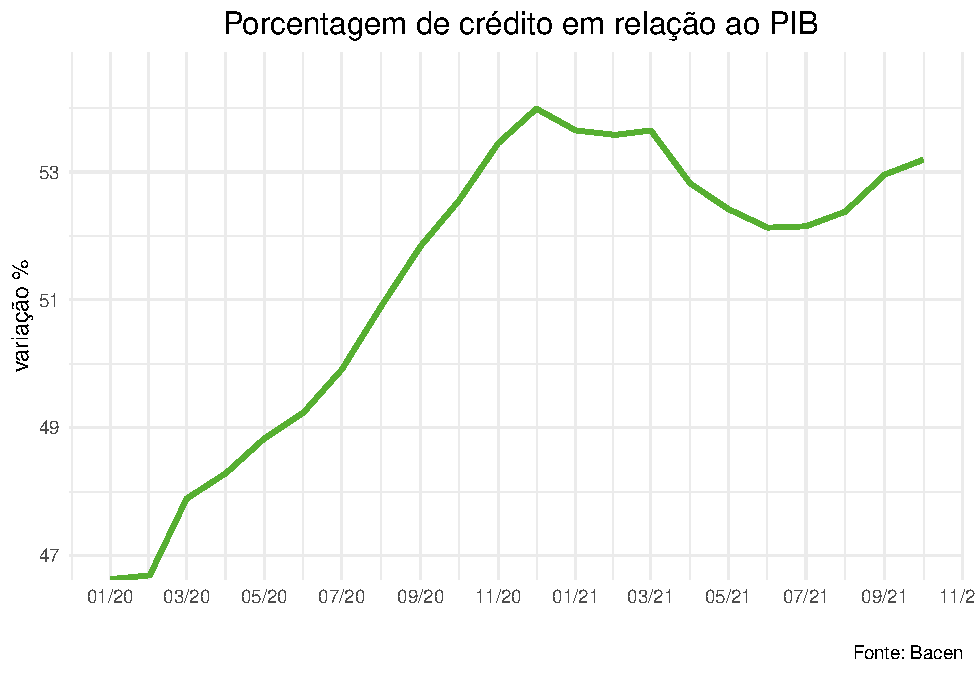
\includegraphics{credito_files/figure-latex/credido e pib-1.pdf}

Em relação ao total das operações de crédito com recursos
livres\footnote{taxas de juros livremente pactuadas entre mutuários e instituições financeiras}
a taxa média de juros situou-se 32,8\% a.a. em outubro, com variação de
2,2\% no mês e 6,3\% em comparação ao mesmo período do ano anterior. No
crédito livre às pessoas jurídicas, a taxa média de juros atingiu 19,1\%
a.a., e para pessoas físicas atingiu 43,8\% a.a., com aumentos de 2,1
p.p. no mês e de 4,8 p.p. em 12 meses.

\newpage

\section{Novas concessões} 
 \vspace{0,15cm}

Em relação ao total de novas contratações, ocorreu retração de 3,8\% em
outubro, com diminuição de 6,1\% nas contratações com pessoas jurídicas,
e queda de 1,7\% nas contratações de pessoas físicas.

\begin{center}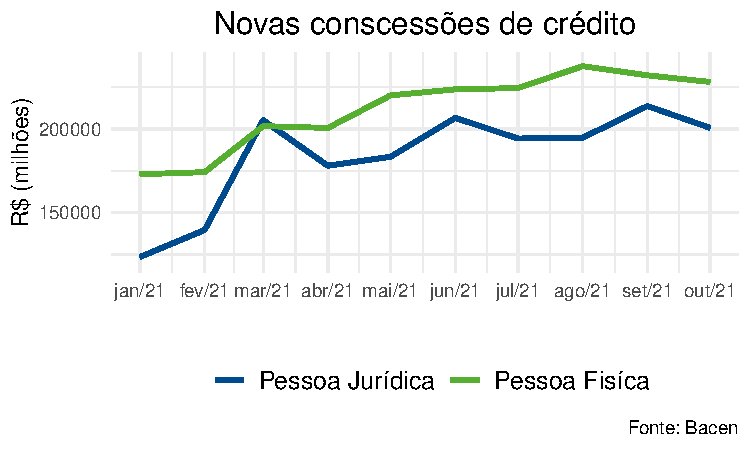
\includegraphics{credito_files/figure-latex/novas conscessoes-1} \end{center}

O valor das novas conscessões de crédito livre às empresas foi de 189,8
bilhões, com queda de 2,2\% em relação ao mês anterior e aumento de
13,5\% no acumulado em doze meses. As altas nas modalidades de
antecipação de faturas de cartão de crédito (5,5\%), capital de giro com
prazo superior a 365 dias (0,9\%) e financiamento às exportações (3,0\%)
se destacam. A concessão de crédito
direcionado\footnote{destinadas principalmente ao investimento de médio e longo prazos, aos setores imobiliário, rural e de infraestrutura.}
atingiu R\$ 34,4 bilhões em outubro, com retração de 44,4\% e retração
interanual de 27,2\%.

Para as pessoas físicas, a concessão de crédito livre foi de R\$ 193,8
bilhões em outubro, queda de 0,2\% em relação ao mês anterior. Em se
tratando do crédito direcionado o valor foi de R\$ 34,4 bilhões, queda
de 9,3\%, em relação ao mês anterior e alta de 42,4\% na comparação
interanual.\footnote{resultados sem ajuste sazonal.}

\newpage
\section{Endividamento das Famílias - Brasil} 
 \vspace{0,15cm}

O endividamento das famílias com o Sistema Financeiro Nacional em
relação à renda acumulada dos últimos doze meses bateu recorde de alta
em junho durante toda série histórica iniciada em 2005, atingiu 59,55\%,
em julho essa porcentagem caiu para 59,24\%

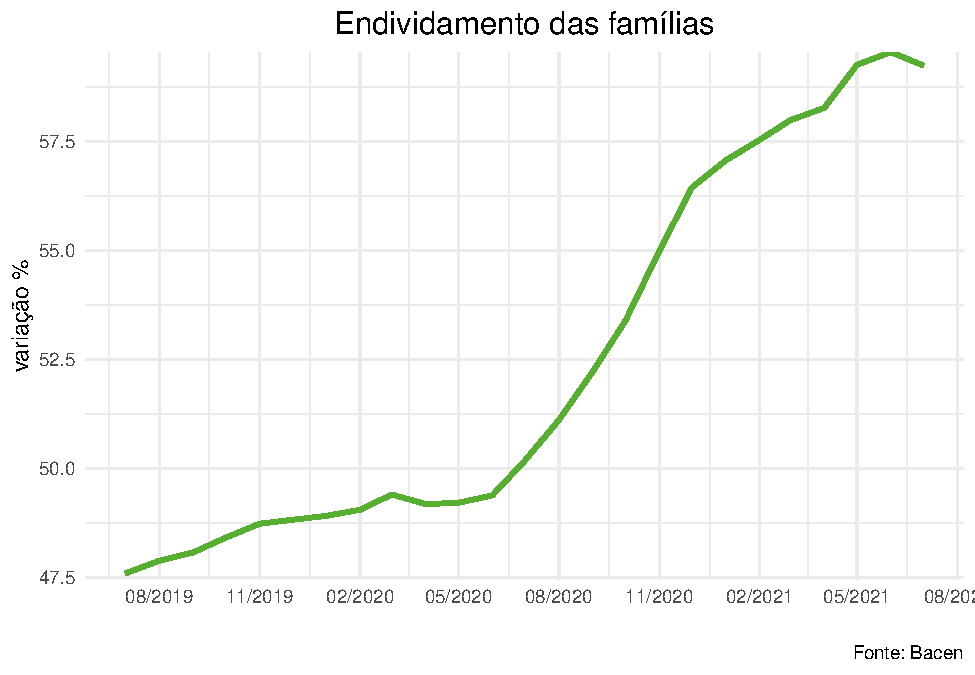
\includegraphics{credito_files/figure-latex/endividamento das familias br-1.pdf}

Esse resultado ocorre principalmente devido ao cenário macroeconômico
brasileiro. A aceleração da taxa de inflação que atingiu 9,26\% no
acumulado do ano diminui o poder de compra das famílias, além disso,
apesar da recente queda na taxa desemprego, ela ainda permanece em um
patamar muito elevado (12,6\%), contribuindo para o endividamento das
famílias. \newpage

\section{ICC e Inadimplência} 
\vspace{0,20cm}

O Indicador de Custo do Crédito (ICC), atingiu 18,0\% a.a., elevando-se
0,3 p.p. no mês e 0,8 p.p. na comparação com outubro de 2020. No crédito
livre não rotativo, o ICC situou-se em 23,7\% a.a., com variações de 0,4
p.p. em outubro e 0,8 p.p. na comparação interanual. Já o spread geral
situou-se em 12,3\% (+0,1 p.p. no mês e +0,2 p.p. na comparação
interanual).

A inadimplência total permaneceu estável em outubro, no patamar de
2,3\%, se mantendo por seis meses consecutivos. Por segmento, o crédito
livre registrou estabilidade neste indicador em 3,0\% do total da
carteira, enquanto nas operações direcionadas a inadimplência apresentou
redução de 0,1 p.p. ao atingir 1,2\%.

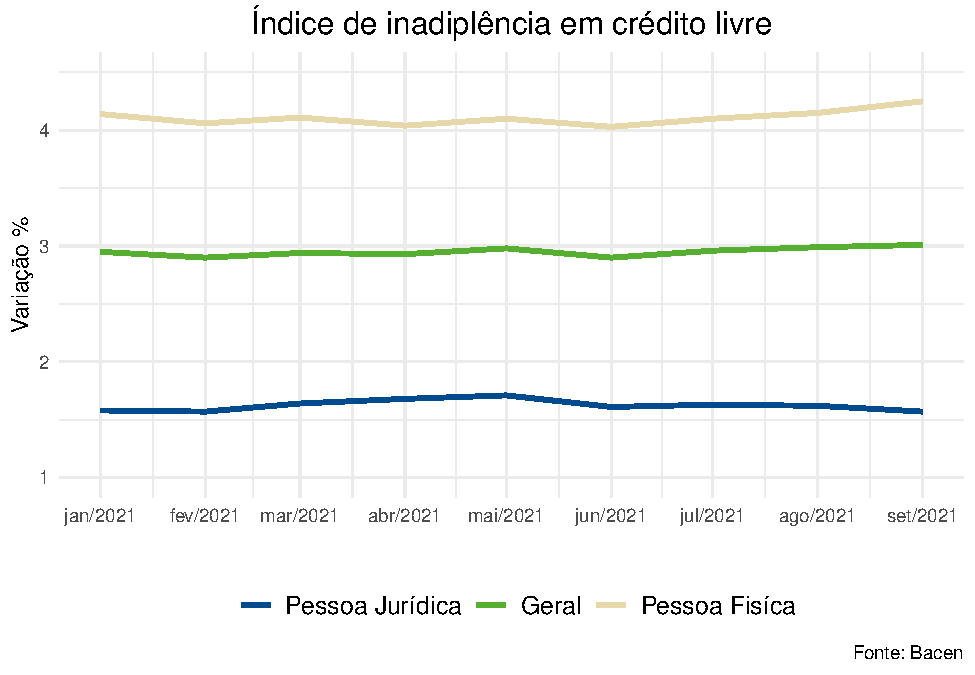
\includegraphics{credito_files/figure-latex/inadimplencia br-1.pdf}

\newpage
\section{Espirito Santo}
\subsection {Saldo nas operações de crédito }
\vspace{0,20cm}

O saldo total de crédito no Espirito Santo em outubro foi de R\$ 68.737
milhões de reais, sendo o crédito destinado às famílias em R\$ 38.131
milhões, e o destinado às pessoas jurídicas em R\$ 30.605 milhões. A
trajetória do saldo de pessoas físicas durante o ano foi bem estável,
enquanto o de pessoas jurídicas teve maior variação.

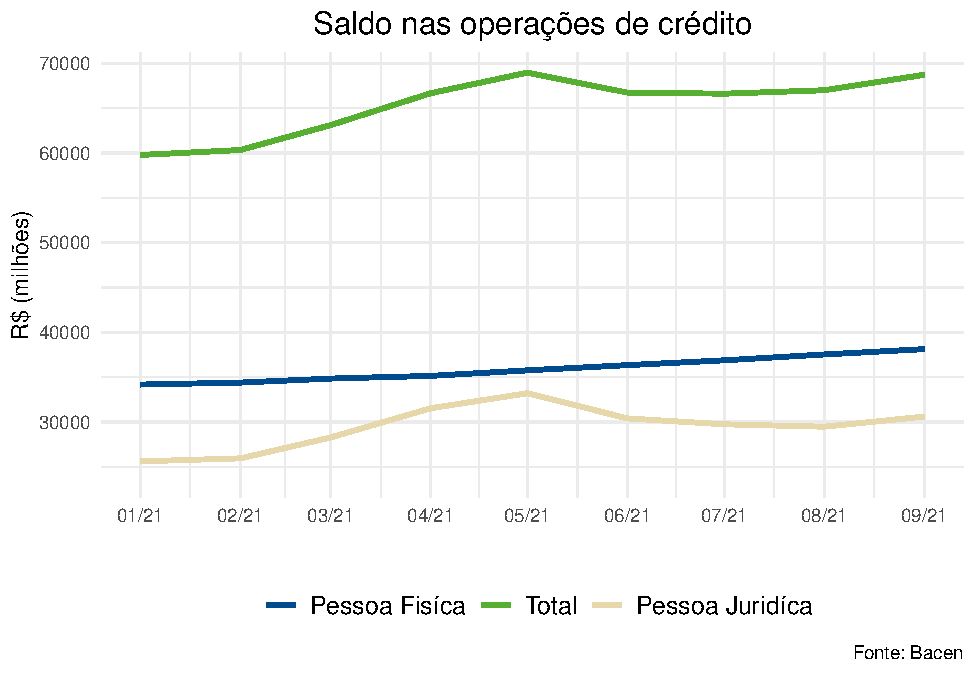
\includegraphics{credito_files/figure-latex/credito es-1.pdf}

\newpage
\subsection {Inadimplência}

A taxa média de inadimplência no Estado se mantém no patamar de 2\%
durante todo ano, com mínima de 1,95\% em janeiro e máxima de 2,23\% em
julho. A partir desse mês a taxa cai influenciada pela queda ascendente
na inadimplência de pessoas jurídicas.

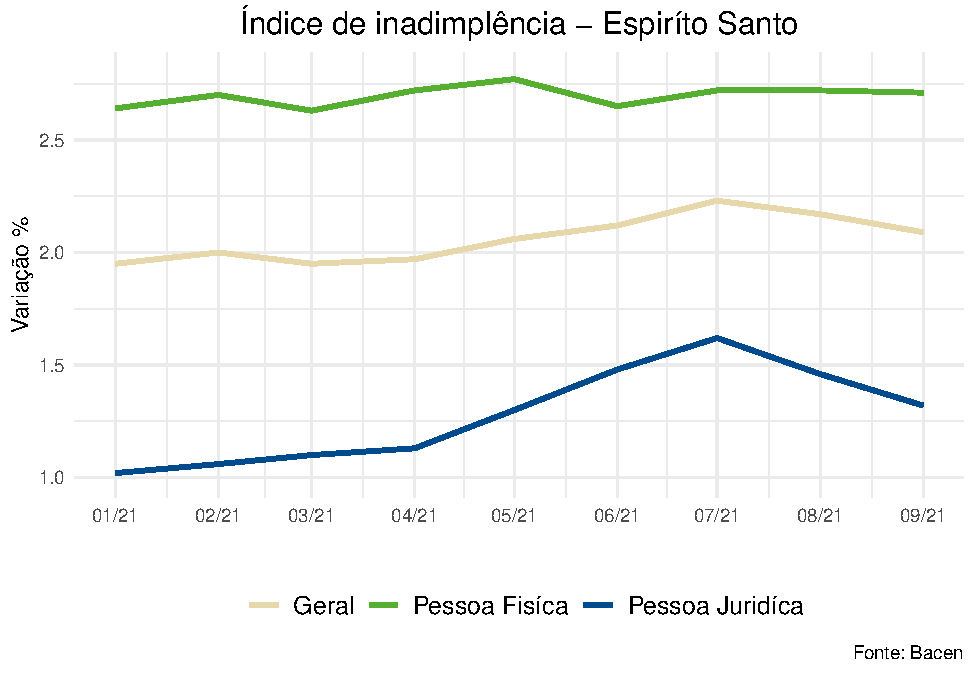
\includegraphics{credito_files/figure-latex/inadimplencia es-1.pdf}


\end{document}
